% \documentclass{standalone}
% \usepackage{tikz}
% \usetikzlibrary{automata, positioning, arrows}

% \begin{document}

% \title{DFA for Character Customization Language}
% \author{}
% \date{}
% \maketitle


% % Begin TikZ diagram for DFA
% \begin{tikzpicture}

%     % Define the states
%     % Start with the initial state (q0)
%     \node[state, initial] (q0) at (0,0) {q0};

%     %for male first path
%     \node[state] (q1) at (3,3) {q1};
%     \node[state] (q2)  at (6,3) {q2};
%     \node[state] (q3)  at (9,3) {q3};

    

%     % %for female second path
%     \node[state] (q4) at (3,-3) {q4};
%     \node[state] (q5) at (6,-3) {q5};
%     \node[state] (q6) at (9,-3) {q6};

%     %accpeting
%     \node[state, accepting] (q7) at (13,0) {q7};


% %drawing now
%     \draw   (q0) edge[bend left, above] node{M} (q1)
%             (q0) edge[bend right, below] node{F} (q4)
%             (q1) edge[loop above] node{MF1,MF2,MF3} (q1)
%             (q1) edge[above] node{MF1..MF3} (q2)
%             (q2) edge[loop above] node{MH1..MH5} (q2)
%             (q2) edge[above] node{MH1..MH5} (q3)
%             (q3) edge[loop right  ] node{HCM1..HCM5} (q3)










% \end{tikzpicture}
% % % End of TikZ diagram for DFA

% \end{document}



%Ignore the above code, its for my reference on understanding the tikz code and implement DFA without using the online resource



%resource used for the code below : https://matthewscholefield.github.io/fsm/
\documentclass[12pt]{article}
\usepackage{tikz}

\begin{document}


\begin{center}
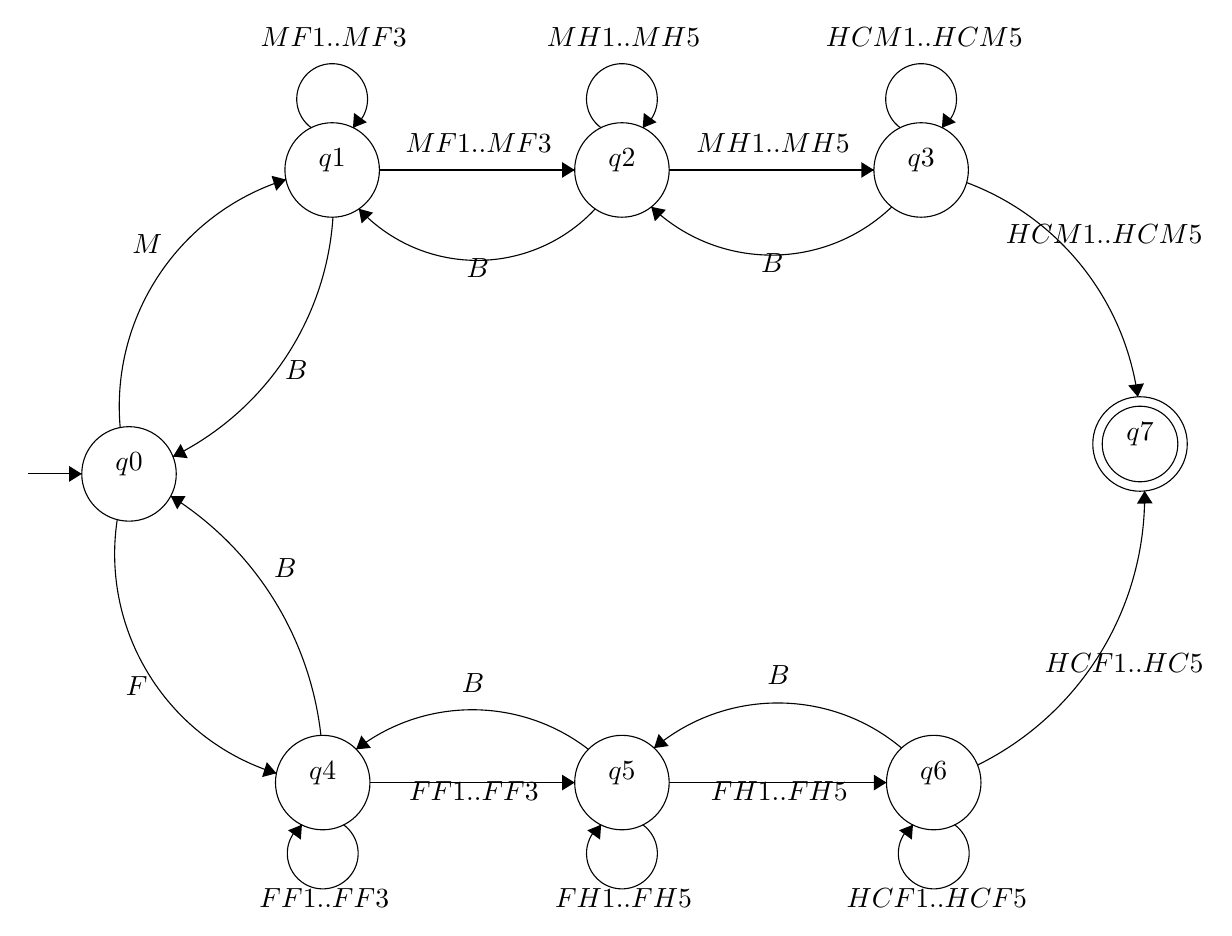
\begin{tikzpicture}[scale=0.2]
\tikzstyle{every node}+=[inner sep=0pt]
\draw [black] (32,-42) circle (3);
\draw (32,-41.4) node {$q0$};
\draw [black] (44.9,-22.7) circle (3);
\draw (44.9,-22.1) node {$q1$};
\draw [black] (44.3,-61.6) circle (3);
\draw (44.3,-61) node {$q4$};
\draw [black] (63.3,-22.7) circle (3);
\draw (63.3,-22.1) node {$q2$};
\draw [black] (63.3,-61.6) circle (3);
\draw (63.3,-61) node {$q5$};
\draw [black] (83.1,-61.6) circle (3);
\draw (83.1,-61) node {$q6$};
\draw [black] (96.2,-40.1) circle (3);
\draw (96.2,-39.5) node {$q7$};
\draw [black] (96.2,-40.1) circle (2.4);
\draw [black] (82.3,-22.7) circle (3);
\draw (82.3,-22.1) node {$q3$};
\draw [black] (31.44,-39.058) arc (-174.91551:-252.60154:15.102);
\fill [black] (41.97,-23.31) -- (41.05,-23.07) -- (41.35,-24.02);
\draw (34.14,-27.4) node [left] {$M$};
\draw [black] (47.9,-22.7) -- (60.3,-22.7);
\fill [black] (60.3,-22.7) -- (59.5,-22.2) -- (59.5,-23.2);
\draw (54.2,-21.6) node [above] {$MF1..MF3$};
\draw [black] (41.363,-61.013) arc (-107.19399:-188.58527:14.588);
\fill [black] (41.36,-61.01) -- (40.75,-60.3) -- (40.45,-61.25);
\draw (33.21,-55.5) node [left] {$F$};
\draw [black] (47.3,-61.6) -- (60.3,-61.6);
\fill [black] (60.3,-61.6) -- (59.5,-61.1) -- (59.5,-62.1);
\draw (53.9,-61.5) node [below] {$FF1..FF3$};
\draw [black] (66.3,-61.6) -- (80.1,-61.6);
\fill [black] (80.1,-61.6) -- (79.3,-61.1) -- (79.3,-62.1);
\draw (73.3,-61.5) node [below] {$FH1..FH5$};
\draw [black] (96.489,-43.083) arc (1.02026:-63.72836:19.033);
\fill [black] (96.49,-43.08) -- (96,-43.89) -- (97,-43.87);
\draw (90.12,-54) node [right] {$HCF1..HC5$};
\draw [black] (85.188,-23.499) arc (69.46681:7.77245:16.984);
\fill [black] (96.06,-37.11) -- (96.45,-36.25) -- (95.45,-36.38);
\draw (87.64,-26.8) node [right] {$HCM1..HCM5$};
\draw [black] (66.3,-22.7) -- (79.3,-22.7);
\fill [black] (79.3,-22.7) -- (78.5,-22.2) -- (78.5,-23.2);
\draw (72.9,-21.6) node [above] {$MH1..MH5$};
\draw [black] (43.577,-20.02) arc (234:-54:2.25);
\draw (45,-14.9) node [above] {$MF1..MF3$};
\fill [black] (46.22,-20.02) -- (47.1,-19.67) -- (46.29,-19.08);
\draw [black] (61.977,-20.02) arc (234:-54:2.25);
\draw (63.4,-14.9) node [above] {$MH1..MH5$};
\fill [black] (64.62,-20.02) -- (65.5,-19.67) -- (64.69,-19.08);
\draw [black] (80.977,-20.02) arc (234:-54:2.25);
\draw (82.5,-14.9) node [above] {$HCM1..HCM5$};
\fill [black] (83.62,-20.02) -- (84.5,-19.67) -- (83.69,-19.08);
\draw [black] (45.623,-64.28) arc (54:-234:2.25);
\draw (44.4,-68.3) node [below] {$FF1..FF3$};
\fill [black] (42.98,-64.28) -- (42.1,-64.63) -- (42.91,-65.22);
\draw [black] (64.623,-64.28) arc (54:-234:2.25);
\draw (63.4,-68.3) node [below] {$FH1..FH5$};
\fill [black] (61.98,-64.28) -- (61.1,-64.63) -- (61.91,-65.22);
\draw [black] (84.423,-64.28) arc (54:-234:2.25);
\draw (83.3,-68.3) node [below] {$HCF1..HCF5$};
\fill [black] (81.78,-64.28) -- (80.9,-64.63) -- (81.71,-65.22);
\draw [black] (44.951,-25.696) arc (-3.73215:-63.78489:18.274);
\fill [black] (34.79,-40.9) -- (35.73,-41) -- (35.28,-40.1);
\draw (41.88,-35.4) node [right] {$B$};
\draw [black] (61.609,-25.165) arc (-42.8515:-137.1485:10.242);
\fill [black] (46.59,-25.16) -- (46.77,-26.09) -- (47.5,-25.41);
\draw (54.15,-28.3) node [below] {$B$};
\draw [black] (80.438,-25.041) arc (-46.27049:-133.72951:11.05);
\fill [black] (65.16,-25.04) -- (65.39,-25.96) -- (66.09,-25.23);
\draw (72.85,-28) node [below] {$B$};
\draw [black] (65.338,-59.409) arc (130.03368:49.96632:12.222);
\fill [black] (65.34,-59.41) -- (66.27,-59.28) -- (65.63,-58.51);
\draw (73.25,-55.4) node [above] {$B$};
\draw [black] (46.423,-59.492) arc (127.67626:52.32374:12.069);
\fill [black] (46.42,-59.49) -- (47.36,-59.4) -- (46.75,-58.61);
\draw (53.85,-55.9) node [above] {$B$};
\draw [black] (34.648,-43.405) arc (57.87783:6.3429:20.639);
\fill [black] (34.65,-43.41) -- (35.06,-44.25) -- (35.59,-43.41);
\draw (41.18,-48) node [right] {$B$};
\draw [black] (25.6,-42) -- (29,-42);
\fill [black] (29,-42) -- (28.2,-41.5) -- (28.2,-42.5);
\end{tikzpicture}
\end{center}

\end{document}
